\chapter{Clustering : Multiple Input Heuristic}\label{section-clustering}

The multi-input transaction clustering heuristic as introduced in section \ref{background:multi-input-tx} and as described in the paper 'A fistful of bitcoins...' \cite{RefWorks:doc:5c3de7e3e4b0ea6196452d80} is one of the simpler, yet most effective clustering heuristics for Bitcoin. In this section, I present the several implementations of the clustering algorithm which uses the same input heuristic. I attempted clustering with many different approaches due to issues discovered while running each clustering algorithm. We also present the successful implementation in section \ref{clustering-raw-csv}.

\section{Java Algorithm using Spring Data}
I implemented an algorithm which performed this clustering in Java; this used the Spring Data interface to the database to fetch all transactions in the database. For each transaction, it then fetches each input and the address each input is locked to. For those transactions with several inputs, each locked to a distinct address, each address is fetched and the set of addresses for the particular transaction are identified as a cluster and therefore under the control of the same user, using this heuristic. To represent this clustering in the database, every address in the cluster will be connected to every other address in the cluster, in a totally connected graph style, using a new relationship type \texttt{INPUT\_HERUISTIC\_LINKED\_ADDRESS}. 
\\\\
The result of running this clustering algorithm for a subset of the database (blocks 0-2000 only) can be seen in figure \ref{fig:neo4j-many-heuristic-1-clusters} and \ref{fig:neo4j-1-tx-heuristic-1-cluster}. 

\begin{figure}[h!]
  \centering
  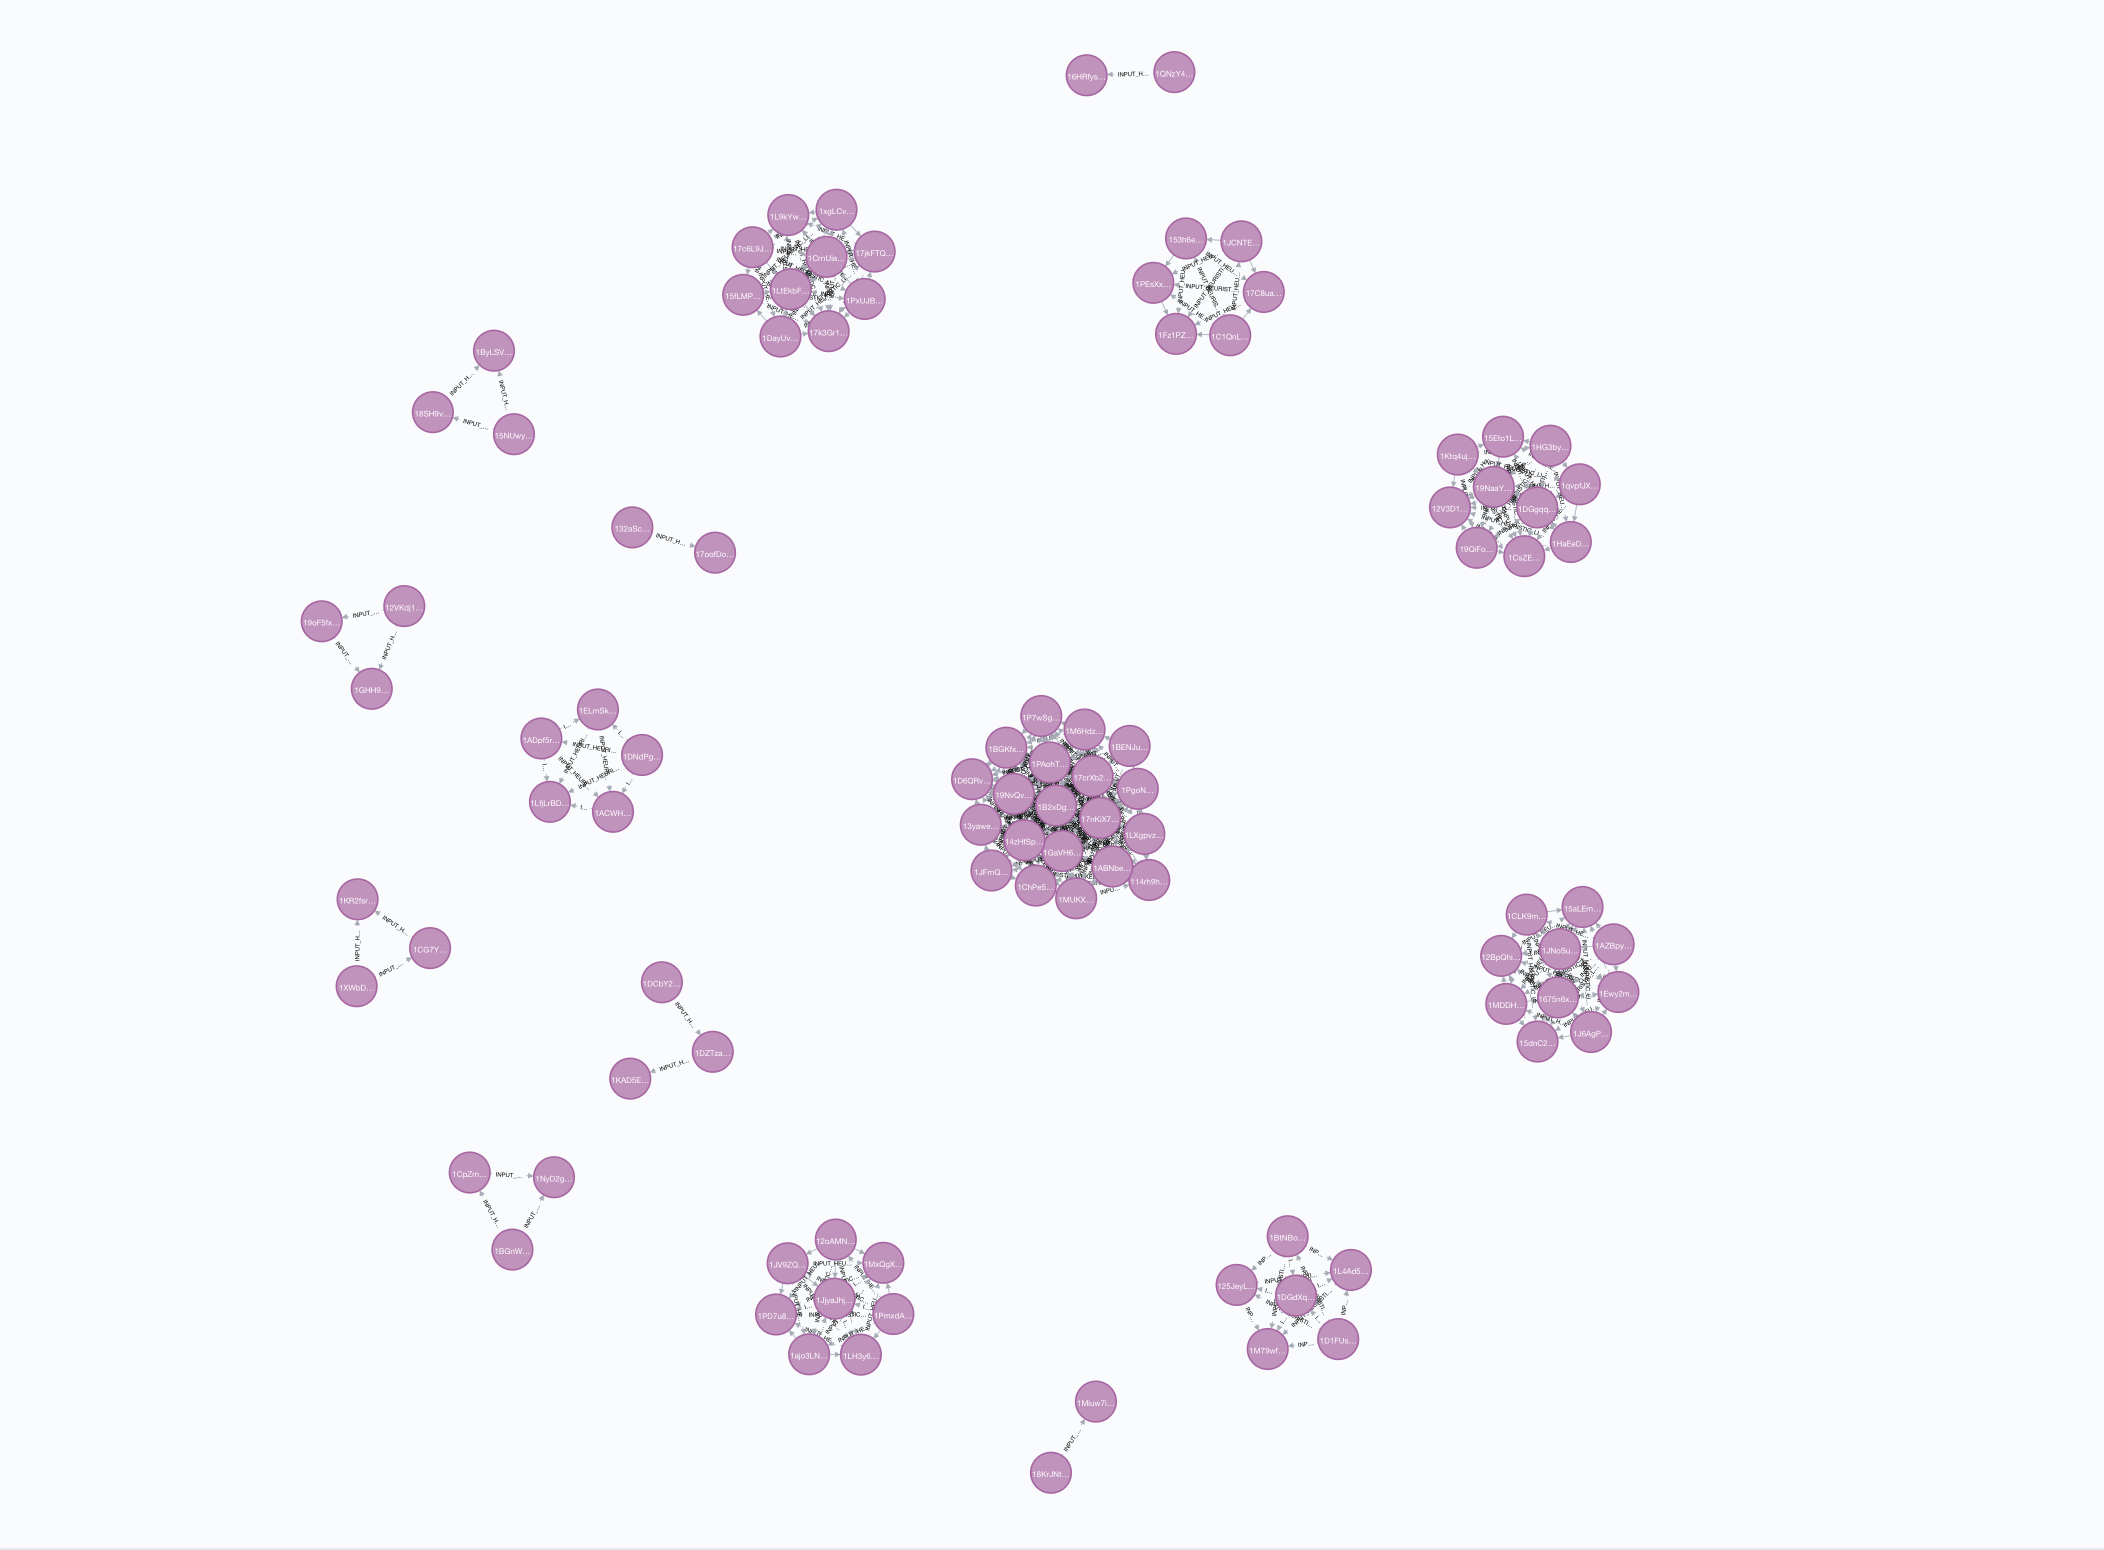
\includegraphics[width = 10cm]{./figures/many-clusters-heuristic-1}\\[0.5cm] 
  \caption{Neo4J browser view of the several clusterings of addresses which all feed the same transaction.}
  \label{fig:neo4j-many-heuristic-1-clusters}
\end{figure}

\begin{figure}[h!]
  \centering
  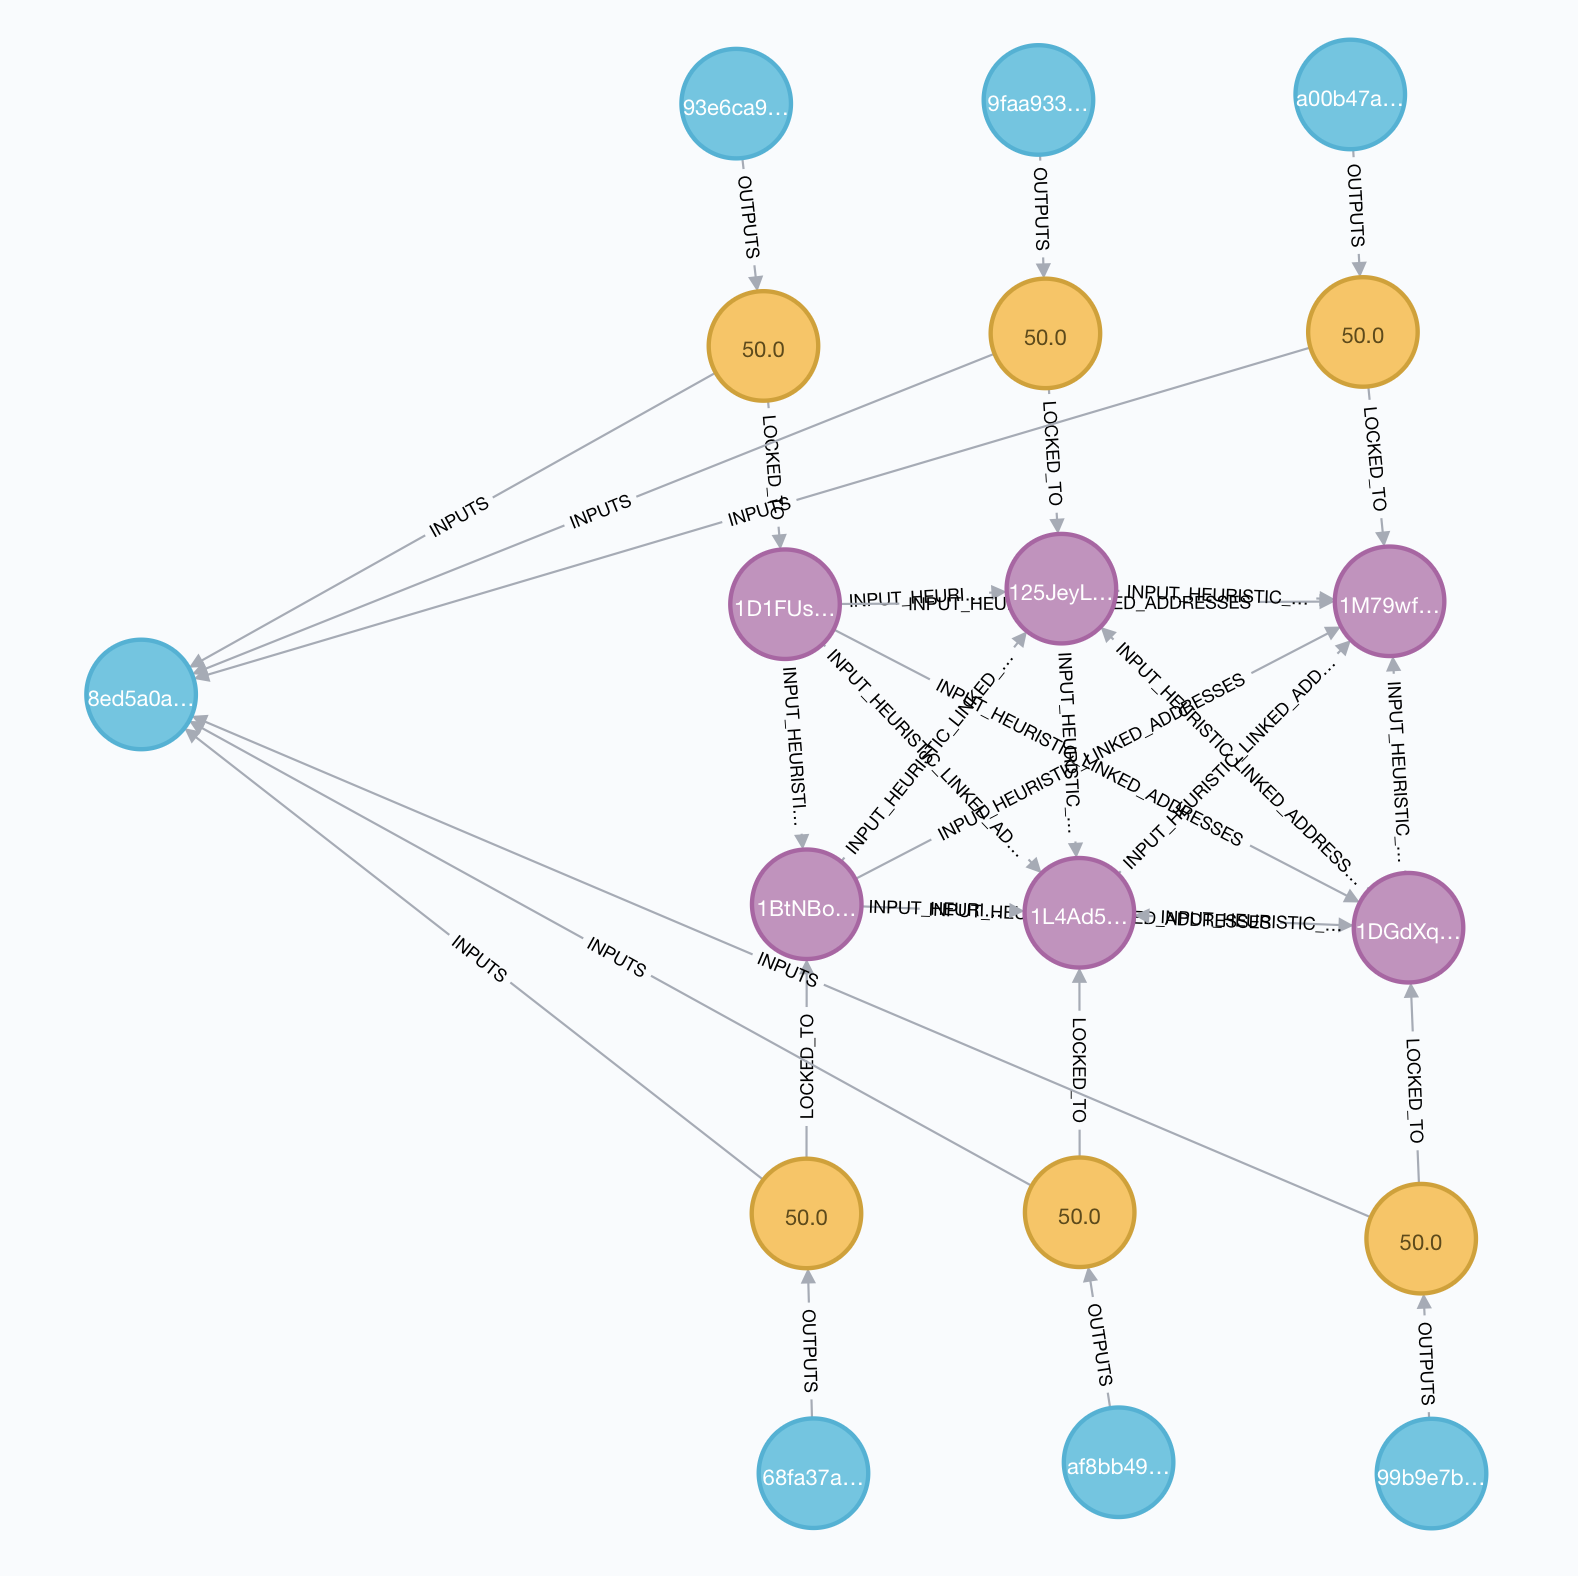
\includegraphics[width = 10cm]{./figures/input-one-tx-heuristic-1}\\[0.5cm] 
  \caption{Neo4J browser view one one of the clusterings of addresses with their neighbours expanded to show they all have outputs locked to them which feed the same transaction}
  \label{fig:neo4j-1-tx-heuristic-1-cluster}
\end{figure}


\subsection{Challenges}

I anticipated the first issue I encountered due to to the size of the dataset I am working with; I encountered a memory overflow error while the algorithm was attempting to load all transactions in Bitcoin into memory. 
\\\\
I solved this issue using Paging. It is possible using Spring Data to use Paging for large requests; I used this to fetch transactions in more granular batches which could be processed before fetching the next batch. This helped tackle memory constraints as the algorithm didn't need to load \textbf{all} transactions up front. See code in Listing \ref{lst:clustering-java}
\\\\
Although progress was being made more steadily using paging, I still experienced performance issues while trying to cluster all addresses for the blockchain. After running the above algorithm for 24 hours, only 150,000 transactions had been processed. This was infeasibly slow, most likely due to the overhead of using Spring Data to fetch every transaction and every Output for the transaction and writing back new relations between each clustered address; I now needed to find a more efficient alternative approach. 
\\\\

\begin{lstlisting}[caption={Java Implementation using Paging}, label={lst:clustering-java}, language=Java, breaklines=true, basicstyle=\small]
public ResponseEntity clusterByInput() {
    //Pageable item: start at page 0, fetch 50 items
    Pageable pageable = PageRequest.of(0, 50);

    while (true) {
        //Fetches transactions for this page
        Page<Transaction> allTransactions = transactionRepository.findAll(pageable);
        allTransactions.forEach(transaction -> {
            
            if (transaction.getInputs() == null || transaction.getInputs().size() < 2) {
                //coinbase input or only one input
                return;// just skips this iteration only
            }
            //Fetch inputs for this transaction
            List<InputRelation> transactionInputs = transaction.getInputs();
            Set<Address> addressesSpendingTransactionInputs = new HashSet<>();

            transactionInputs.forEach(inputRelation -> {
                String inputId = inputRelation.getInput().getOutputId();
                
                //Fetches the entire Output node from the database, so it's
                //relation fields are populated
                Output refetchedTransactionInput = getOutputById(inputId);
                Address addressSpendingTransactionInput = refetchedTransactionInput.getLockedToAddress();
                
                //add every distinct address to a set
                if (addressSpendingTransactionInput != null) {
                    addressesSpendingTransactionInputs.add(addressSpendingTransactionInput);
                }
            });

            //iterate through the set, link every item in set with evrey other
            addressesSpendingTransactionInputs.forEach(address -> {
                address.setInputHeuristicLinkedAddresses(addressesSpendingTransactionInputs);
                
                // Saves the updated addresses back to Neo4J repo at depth 0
                this.addressRepository.save(address, 0);
            });

            System.out.println("completed for tx" + transaction.getTransactionId());

        });

        if (!allTransactions.hasNext()) {
            //reached the last page: terminate
            break;
        }
        
        //fetches the next page to request
        pageable = allTransactions.nextPageable();
    }

    return ResponseEntity.status(200).body("Clustering Complete");
}
\end{lstlisting}

\section{Cypher Query}
I was able to translate the above algorithm in Listing \ref{lst:clustering-java} to a single Cypher query. The Cypher implementation is shown in Listing \ref{lst:clustering-cypher}.
The query matches all transactions that have more than one input, then finds the addresses each input is locked to. It uses the \texttt{UNWIND} commands to generate all pairs of addresses in the address list for a particular transaction. The clause \texttt{WHERE id(first) \< id(second)} ensures a pair of addresses only occurs once; rather than two pairs existing for \{a,b\} and \{b,a\} where a and b are both addresses.

\begin{lstlisting}[caption={Cypher Implementation}, label={lst:clustering-cypher}, breaklines=true, basicstyle=\small]
MATCH (t:TRANSACTION)
WHERE size((t)<-[:INPUTS]-()) > 1
WITH [(t)<-[:INPUTS]-(:OUTPUT)-[:LOCKED_TO]->(a:ADDRESS) | a] as addresses
UNWIND addresses as first
UNWIND addresses as second
WITH addresses, first, second
WHERE id(first) < id(second)
MERGE (first)-[:INPUTS_SAME_TX]-(second)
\end{lstlisting}

Before I could execute the query, I first had to clean up the mutations made to the database by my previous attempt. To do this, I created a Query to delete all instances of the relationship I added in the first attempt. 

I encountered performance issue with my initial delete query. 
The initial query was simply:
\begin{lstlisting}
MATCH (:ADDRESS)-[r:INPUT_HEURISTIC_LINKED_ADDRESSES]-(:ADDRESS)
DELETE r
\end{lstlisting}

\subsection{Performance Issues}
When executing the query shown in Listing \ref{lst:clustering-cypher} I encountered performance issues where several hours would elapse with no apparent progress being made. I investigated this issue using the Cypher \texttt{PROFILE} command to inspect the performance of this query. The performance report identified issues in the earlier stages where the query would require the search of all nodes across the database when matching transactions, inputs and addresses. Since we want to match all nodes, rather than using a specific ID that can leverage fast index lookups, this leads to a significant bottleneck in the query. 
\\\\
Due to the nature of the query I was performing, there was no apparent way to resolve the performance issues with this query. It would simply need to match millions of nodes. Therefore, I investigated an alternative approach, of performing the clustering 'on the fly' as and when an address is requested from the UI. 

\section{Clustering on demand}
By knowing exactly which address we want to perform the clustering for, and leveraging the performance enhancements provided by indexes on address, transactions and outputs when fetching them using their respective ID's, I was able to craft an algorithm to efficiently implement clustering on demand.
\\\\
This implementation heavily relied on Java 8 streams, specifically using parallel streams to take advantage of parallelizability in the tasks to be performed, increasing the efficiency of this operation; critical for an on-demand process. 
\\\\
The implementation of this algorithm led me to discover that my initial implementation (Listing \ref{lst:clustering-java}) was not correct. This heuristic is transitive, such that if addresses A and B input the same transaction, and B and C input the same transaction then A, B and C can all be considered as under the control of the same user. My implementation in Listing \ref{lst:clustering-java} does not take this transitivity into account. However, I ensured transitivity was encountered before in my on-demand clustering algorithm in Listing \ref{lst:clustering-on-demand}.

\begin{lstlisting}[language=Java, caption={Java Implementation of on demand clustering}, label={lst:clustering-on-demand}, breaklines=true, basicstyle=\small]
private void performInputClustering(Address addressNode, Date start, Date end) {
    Set<Address> linkedAddresses = transitiveInputClustering(addressNode, new HashSet<>(), start, end);
    addressNode.setInputHeuristicLinkedAddresses(linkedAddresses);
}

private Set<Address> transitiveInputClustering(Address addressNode, Set<Transaction> exploredTransactions, Date start, Date end) {
    //a stream of transactions which all have inputs locked to this address
    Stream<Transaction> allTransactionsThisAddressInputs = getTransactionsForAddress(addressNode, start, end);
    HashSet<Transaction> thisAddressesTransactions = allTransactionsThisAddressInputs.collect(Collectors.toCollection(HashSet::new));

    //removes all transactions we've already seen
    thisAddressesTransactions.removeAll(exploredTransactions);

    //now adds the new transactions we're about to explore to the explored set
    exploredTransactions.addAll(thisAddressesTransactions);

    //all addresses linked directly (1 transaction hop away) from this address
    Stream<Address> linkedAddressesStream = getAddressesLinkedByTransactions(thisAddressesTransactions.parallelStream(), start, end);
    Set<Address> directlyLinkedAddresses = linkedAddressesStream.collect(Collectors.toSet());

    //all addresses linked transitively (2 transaction hops away) from this address
    Stream<Set<Address>> transitiveAddressStream = directlyLinkedAddresses
            .stream()
            .map(linkedAddress -> transitiveInputClustering(linkedAddress, exploredTransactions, start, end));
    directlyLinkedAddresses.addAll(transitiveAddressStream.flatMap(Set::stream).collect(Collectors.toSet()));

    return directlyLinkedAddresses;
}

private Stream<Transaction> getTransactionsForAddress(Address address, Date start, Date end) {
    return address.getOutputs()
            .parallelStream()
            .map(outputShell -> findOutputNode(outputShell.getOutputId(), start, end))
            .filter(outputNode -> outputNode.getInputsTransaction() != null)
            .map(outputNode -> outputNode.getInputsTransaction().getTransaction())
            .map(transactionShell -> findTransaction(transactionShell.getTransactionId()))
            .filter(transactionNode -> transactionNode.getInputs() != null && transactionNode.getInputs().size() > 1);
}

private Stream<Address> getAddressesLinkedByTransactions(Stream<Transaction> transactionStream, Date start, Date end) {
    return transactionStream.flatMap(tx -> getAddressesLinkedByTransaction(tx, start, end));
}
private Stream<Address> getAddressesLinkedByTransaction(Transaction transaction, Date start, Date end) {
    return transaction.getInputs()
            .parallelStream()
            .map(InputRelation::getInput)
            .map(inputShell -> findOutputNode(inputShell.getOutputId(), start, end))
            .map(Output::getLockedToAddress);
}
\end{lstlisting}

\subsection{Correctness}


I can verify the correctness of clustering by immediate neighbours by searching for a transaction known to have several inputs locked to distinct addresses. For example, I was able to verify the correctness of clustering with immediate neighbours using address \texttt{17jkFTQuYaGssazzqZ6CTHgRVQYRgLmf34}. This address inputs transaction \\\texttt{8897ea9ceaf18a546cdc513b9179bae31a462ee5bf47818eb7ba909082d11777}, and also has inputs from 9 other distinct addresses. The clustering algorithm then produces a cluster of 10 addresses that are considered to be controlled by the same user. 
\\\\
I now verify the transitive clustering behaviour of the algorithm.  
To achieve this, I mutated my local Neo4J database containing a subset of the Bitcoin Blockchain (only blocks 0-2000). 
\\\\
I manually located an instance of addresses that can be clustered transitively using this heurisitc. The visual representation of the connections existing between two transitively linked addresses can be seen in figure \ref{fig:neo4j-transitive-clustering-screenshot}. The 3 addresses in this screenshot (in green) are \texttt{15oUEZFKAC8E8BTLt1s1jx4fPxumwB3ecr}, \texttt{17iqXQcGfjjHSsJK993mu75sPBnLFSEp8F} and \texttt{1Js6Nx1822qSjETsnp2kkhQFwmRNRWxgak}. They are linked through two transactions (in blue) \texttt{04dc7226529763e8c15d58171d1ac1e28cb6b8d3165005765e65757c7b219d2d} and \texttt{c7a4bb767027a4382462c32b6a824a53e2715d833c0d86e9676a4fbddedca0a9}. 
\\\\
I was able to verify that executing the clustering algorithm included all 3 of these addresses in the result, and became confident of the correct transitive behaviour of my implementation of the clustering algorithm. 

\begin{figure}[h!]
  \centering
  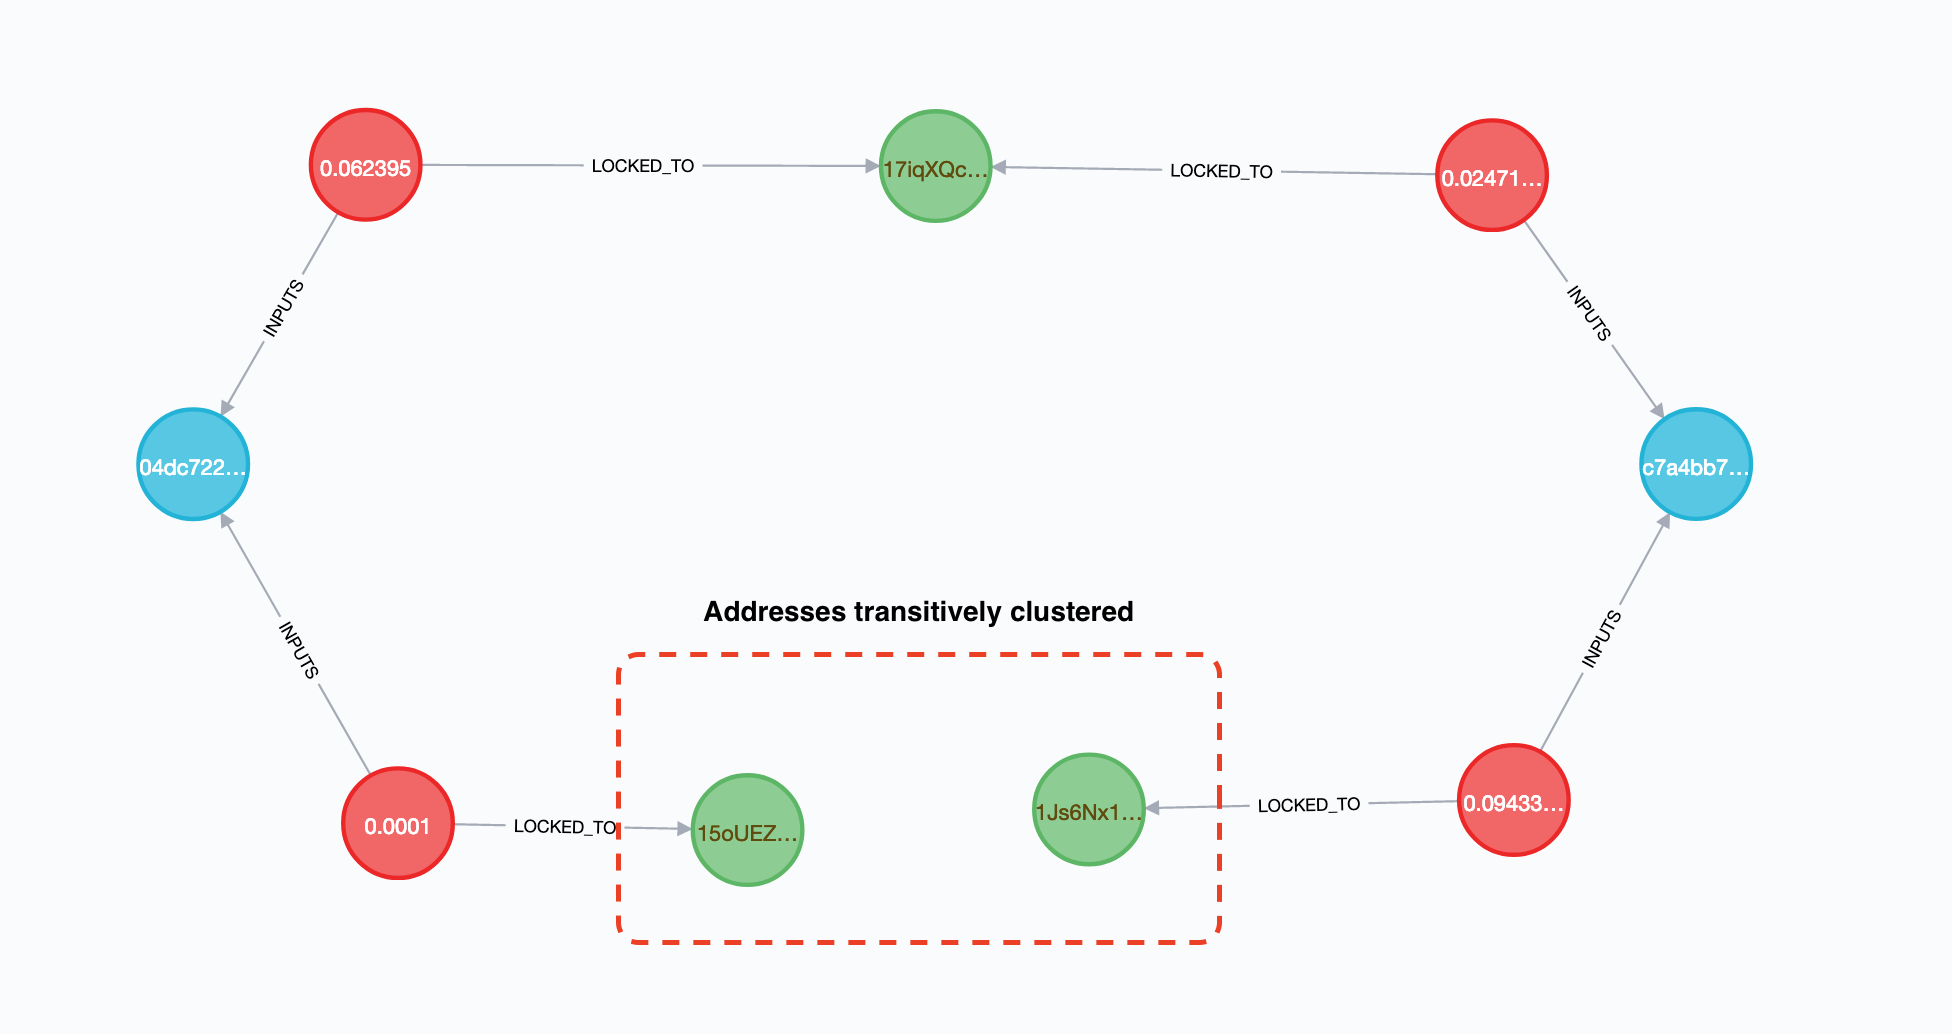
\includegraphics[width = 15cm]{./figures/neo4j-screenshots/addresses-transitively-clustered}\\[0.5cm] 
  \caption{A screenshot of the Neo4J UI : Visual representation of addresses that are clustered transitively.}
  \label{fig:neo4j-transitive-clustering-screenshot}
\end{figure}

\subsection{Drawbacks \& Compromises}
On-demand clustering begins to become unsuitable for extremely large clusters; for example, an address belonging to the wallet of SatoshiDice.com \\\texttt{1LaM2aDLEP49kLbE6y2hvnbrP3agbMwEHb} would belong to an extremely large cluster of many thousands of addresses, and clustering on-demand would simply take far too long to provide an acceptable user experience (I experimented with the above address and killed the request after 30 minutes had elapsed). For addresses belonging to large wallets like the one above, I attempt to cluster using the entity tagging information obtained in section \ref{section-entity-tagging} rather than using the multi-input heuristic.
Since this data is stored in the database, it is quick to traverse the \texttt{HAS\_ENTITY} relationships from a known address to find all of the addresses in the cluster. Therefore, I prioritise providing entity clustering information over input clustering in order to provide as much valuable information over a shorter time; improving user experience. \\\\
For those addresses that do not have a link with a known entity, but exist as part of large address clusters, I constrain the search for linked addresses. After finding a specified number of linked addresses, the search for further addresses will complete and return a subset of the cluster to the user. The limit is configurable on the search form and the user has the ability to disable the limit in order to find the complete result, but with the warning that it could be a time-consuming operation. I feel this was a suitable compromise to make in order to provide the clustering functionality while also maintaining good user experience. 


\section{Clustering using raw CSV data}\label{clustering-raw-csv}
Due to the challenges experienced in the earlier approaches, where clustering relations were added once the Neo4J database had already been populated and hence was, a different approach was required where the clustering would be performed by generating new CSV relations to be used in the bulk import described in section \ref{section-blockchain-import}. 
\\\\
If the clustered addresses could be represented as relationships in the graph, where each address will be a neighbour of each address in its cluster, it will be efficient to query the database for addresses in the same cluster of a particular addres;  Neo4J is designed to traverse large number of relationships extremely quickly. This approach was attempted in the first two implementations documented in this section, however these approaches had the constraint of the transnational layer above the database causing the clustering algorithm to be very slow. By working with raw CSV data, we are able to circumvent this issue and leverage the powerful Neo4J Import tool used to populate the database [see section \ref{section-blockchain-import}] to include these relationships in the initial import. 

\subsection{Approach}
The idea of this approach is to generate a CSV file for the relationships representing addresses that should be clustered together. Each entry in the CSV file will have the format \texttt{ADDRESS\_IN\_CLUSTER, ANOTHER\_ADDRESS\_IN\_CLUSTER, INPUTS\_SAME\_TX} where \texttt{ADDRESS\_IN\_CLUSTER} and \texttt{ANOTHER\_ADDRESS\_IN\_CLUSTER} are two Bitcoin addresses and \texttt{INPUTS\_SAME\_TX} is the name of the relationship. 
\\\\
The outline of the algorithm is as follows:
\begin{itemize}
    \item for each transaction $tx$ on the Blockchain
    \begin{itemize}
        \item Fetches inputs $ins$ of $tx$
        \item Maps $ins$ to the addresses the input is locked to and generates a set of addresses $as$ which input the transaction 
        \item Writes a new CSV relationship entry for every pair $a1, a2$ in $as$ where $a1 != a2$
    \end{itemize}
    \item The new input relations CSV files are then used in the Neo4J import tool to re-import the entire database, now with clustering information
\end{itemize}
I leveraged concurrency in the implementation of the above algorithm. I implemented the algorithm in Java, splitting the transactions to be iterated through into seperate chunks to be submitted to thread pool workers. I addressed possible race conditions and file lock contentions by having each thread writing to its own output CSV file.  

